\documentclass[10pt,a4paper]{article}
\usepackage[margin=18mm]{geometry}
\usepackage[T1]{fontenc}
\usepackage{lmodern,microtype,amsmath,booktabs,graphicx,xcolor,float,tabularx,array}
\setlength{\parindent}{0pt}
\setlength{\parskip}{5pt}
\newcommand{\good}[1]{\textcolor{green!45!black}{#1}}
\newcommand{\snapshot}{\textsuperscript{\dag}}
\begin{document}

\begin{center}
{\Large\bfseries Selectime: validation-selected input and retrieval mixtures}\\[4pt]
30 September 2026
\end{center}

\section*{Evidence status}

The completed comparison contains 90 matched TIME tasks and 67,502
Seasonal-defined metric rows per method. The numerical tables and figures in
this report describe the completed artifact snapshot published as Git revision
\texttt{924bece57}. They are marked \snapshot{} because two subsequently
implemented calibration gates---minimum validation support and minimum
empirical alternative win rate---have not yet been applied to the saved
results. Candidate forecasts remain reusable, but calibration, assembly,
evaluation, and reporting must be regenerated before these values become the
current gated result.

\section*{Main findings from the completed pre-gate snapshot}

Chronos-2 scope mixing was strongest overall. The per-variate scope mixture
reduced mean task MASE by \good{1.013\%} relative to univariate input, while the
task scope mixture had the best task win rate at 80.0\%. Native multivariate
input remained competitive at \good{0.958\%}. Among retrieval mixtures,
$K=5$ was best in aggregate at \good{0.363\%}; its advantage was concentrated
on medium and long horizons. No single $K$ dominated every
frequency--horizon cell.

Chronos-Bolt reported only vanilla univariate forecasting because its backbone
does not accept non-empty covariates or multivariate histories. Its mean task
MASE was 1.167905, 9.23\% above univariate Chronos-2. This is a backbone
comparison, not evidence that the Selectime controls were tested on Bolt.

\begin{figure}[H]
\centering
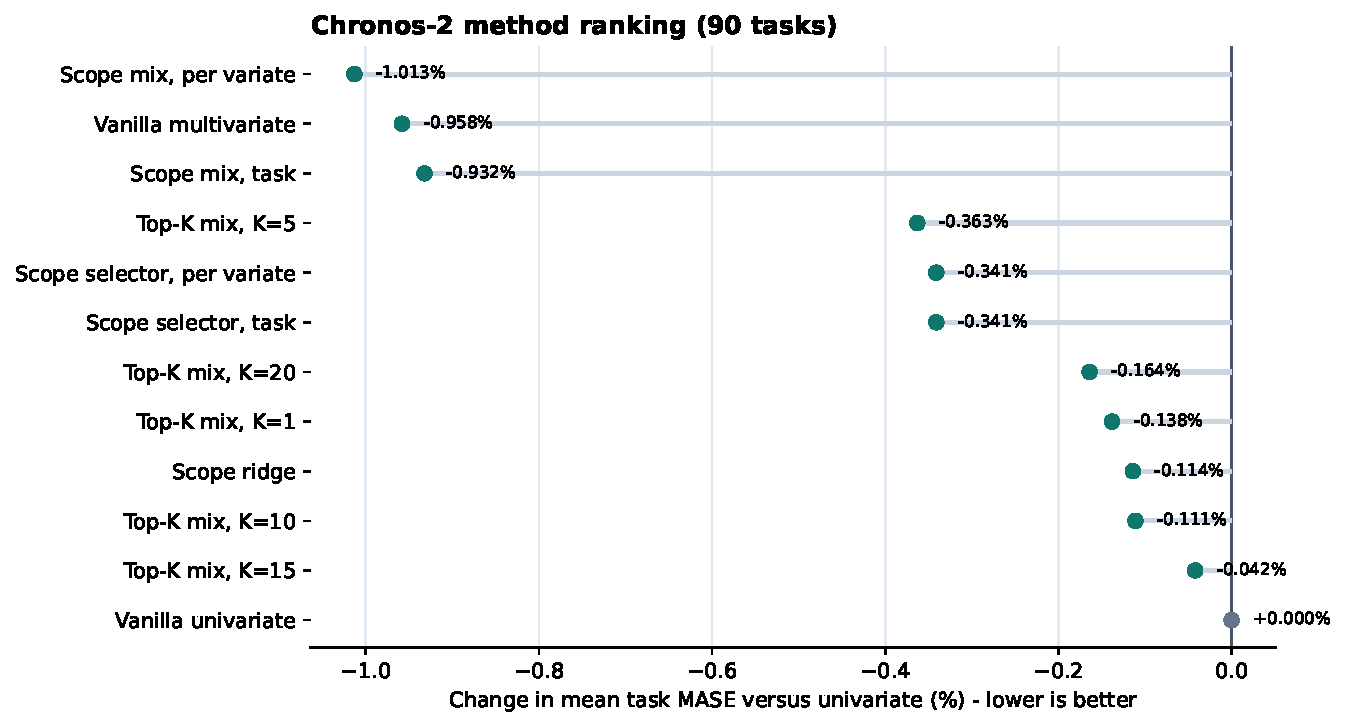
\includegraphics[width=.94\textwidth]{assets/method_ranking.pdf}
\caption{Completed pre-gate Chronos-2 ranking. Negative change means lower mean
task MASE than univariate Chronos-2. Every method gives equal weight to each of
the 90 task means.}
\end{figure}

\section{Question and reduced protocol}

For target history $x$ and horizon-$H$ future $y$, let $V$ be the frozen
univariate forecast and $M$ the native multivariate Chronos-2 forecast. For
$K\in\{1,5,10,15,20\}$, retrieve the $K$ closest aligned historical windows by
instance-normalized lookback distance. Rescale their histories and already
observed futures using lookback-only statistics, then supply them as past and
future covariate channels to obtain $R_K$. A reported retrieval mixture is
\[
  \widehat y_K=(1-p_K)V+p_KR_K.
\]
Scope mixtures replace $R_K$ with $M$ and fit one task-level or item/variate
weight. Hard scope selectors choose $V$ or $M$; scope ridge fits
$V+p(M-V)$ with fixed $\alpha=1$ and does not clip $p$.

In the completed snapshot, a heuristic mixture with $w$ validation wins in
$n$ eligible validation rows used the Beta$(1,1)$ posterior mean
$p=(1+w)/(2+n)$; ties contributed half a win. A task-level weight uses only
that task. A per-variate weight uses only the corresponding item/variate.
Rows where the alternative fell back to univariate were excluded rather than
counted as ties. The canonical univariate forecast has no fallback path and
must be finite.

The current unexecuted contract additionally requires
\[
 n\ge 10,\qquad n/N_{\mathrm{test}}>0.10,\qquad w/n>0.10.
\]
Otherwise $p=0$ and the reported forecast is exactly $V$. Here
$N_{\mathrm{test}}$ counts matching forecast rows at the same task or
item/variate granularity.

\section{Exact leading results}

\begin{center}
\small
\begin{tabularx}{\textwidth}{@{}rXrrr>{\raggedright\arraybackslash}p{45mm}@{}}
\toprule
Rank & Method & Mean MASE & Improvement & Win rate & Recorded inference\\
\midrule
1 & Scope mix, per variate\snapshot & 1.058395 & \good{+1.013\%} & 71.1\% & Assembled; no independent latency\\
2 & Vanilla multivariate & 1.058981 & \good{+0.958\%} & 57.8\% & 87.1 s summed query-loop time\\
3 & Scope mix, task\snapshot & 1.059264 & \good{+0.932\%} & \textbf{80.0\%} & Assembled; no independent latency\\
4 & Top-$K$ mix, $K=5$\snapshot & 1.065347 & \good{+0.363\%} & 56.7\% & Assembled; no independent latency\\
5 & Scope selector, per variate & 1.065584 & \good{+0.341\%} & 41.1\% & Assembled; no independent latency\\
\bottomrule
\end{tabularx}
\end{center}

Improvement is $100(1-\mathrm{MASE}_{m}/\mathrm{MASE}_{V})$, so positive is
better. Win rate is the strict fraction of the 90 task MASE values below the
univariate task value; ties remain in the denominator. Assembled methods reuse
candidate artifacts and therefore have no measured cold inference latency.

\begin{figure}[H]
\centering
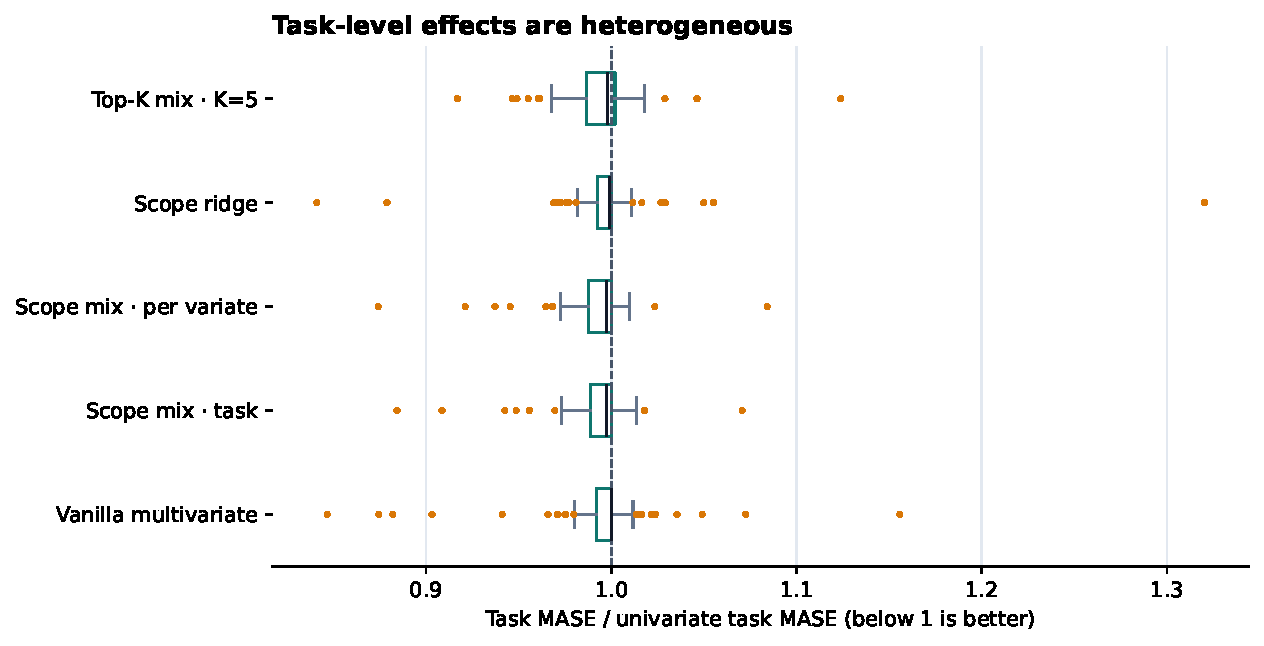
\includegraphics[width=.9\textwidth]{assets/task_ratio_boxplot.pdf}
\caption{Paired task ratios reveal heterogeneous effects hidden by aggregate
means. Values below one improve on univariate; the boxes summarize 90 task
ratios and orange points are Tukey outliers.}
\end{figure}

\begin{center}
\small
\begin{tabular}{lrlr}
\toprule
Largest per-variate-mix gains & Improvement & Largest losses & Degradation\\
\midrule
Coastal\_T\_S / 20T / long & +12.58\% & US\_Labor / M / short & 8.43\%\\
Vehicle\_Supply / M / short & +7.88\% & Uncertainty\_1M / M / short & 2.35\%\\
JOLTS / M / short & +6.27\% & EWELD\_Load / 15T / long & 0.96\%\\
Global\_Price / Q / short & +5.46\% & EWELD\_Load / 15T / medium & 0.62\%\\
Housing\_Inventory / M / short & +3.53\% & Coastal\_T\_S / 20T / short & 0.43\%\\
\bottomrule
\end{tabular}
\end{center}

\section{Forecast-term and domain structure}

\begin{figure}[H]
\centering
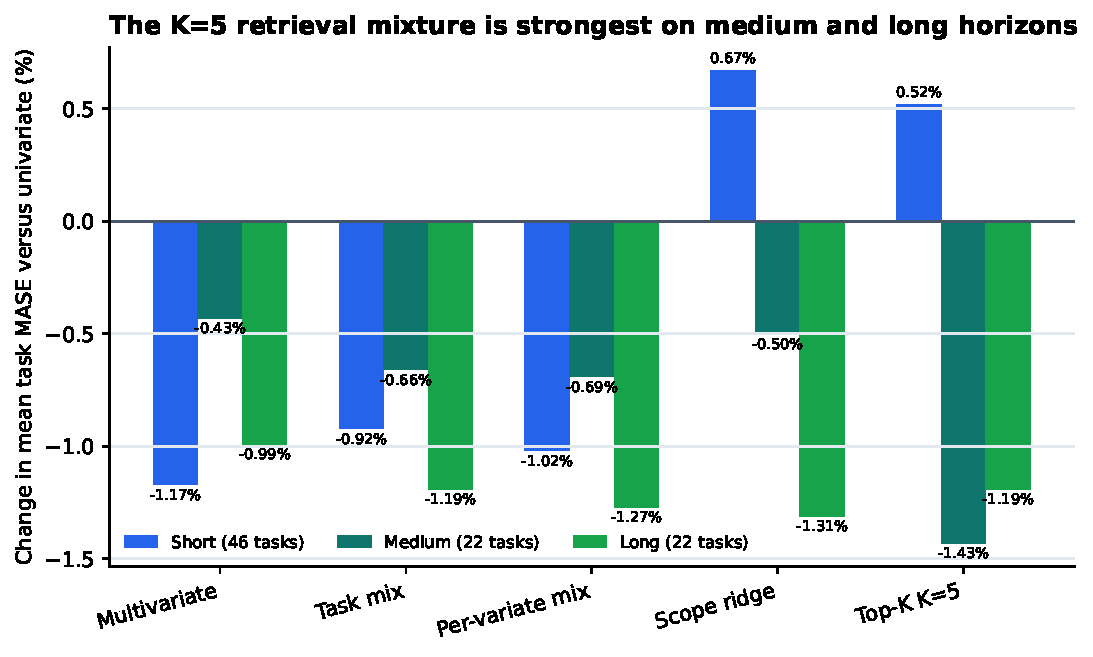
\includegraphics[width=.96\textwidth]{assets/term_breakdown.pdf}
\caption{Completed pre-gate changes by forecast term. The $K=5$ retrieval
mixture degrades the short-term mean by 0.52\%, but improves medium and long
means by 1.43\% and 1.19\%.}
\end{figure}

\begin{center}
\small
\begin{tabular}{lrrrr}
\toprule
Domain & Tasks & Multivariate & Per-variate mix\snapshot & $K=5$ mix\snapshot\\
\midrule
Climate & 45 & +0.84\% & +1.12\% & +1.09\%\\
Economics & 11 & +2.79\% & +2.16\% & $-0.89\%$\\
Transport & 11 & $-0.14\%$ & +0.05\% & +0.26\%\\
Energy & 6 & $-1.02\%$ & +0.26\% & +2.14\%\\
Finance & 6 & +1.64\% & +0.88\% & $-0.22\%$\\
Sales & 4 & $-0.08\%$ & +0.27\% & $-0.28\%$\\
Healthcare & 3 & +0.20\% & +0.46\% & $-1.71\%$\\
Industry & 3 & +0.02\% & +0.02\% & 0.00\%\\
Cloud operations & 1 & $-0.55\%$ & $-0.02\%$ & 0.00\%\\
\bottomrule
\end{tabular}
\end{center}

Positive values in this table mean improvement over univariate. Small-domain
rows are descriptive; they are not separately powered comparisons.

\section{Frequency--horizon winners}

\begin{figure}[p]
\centering
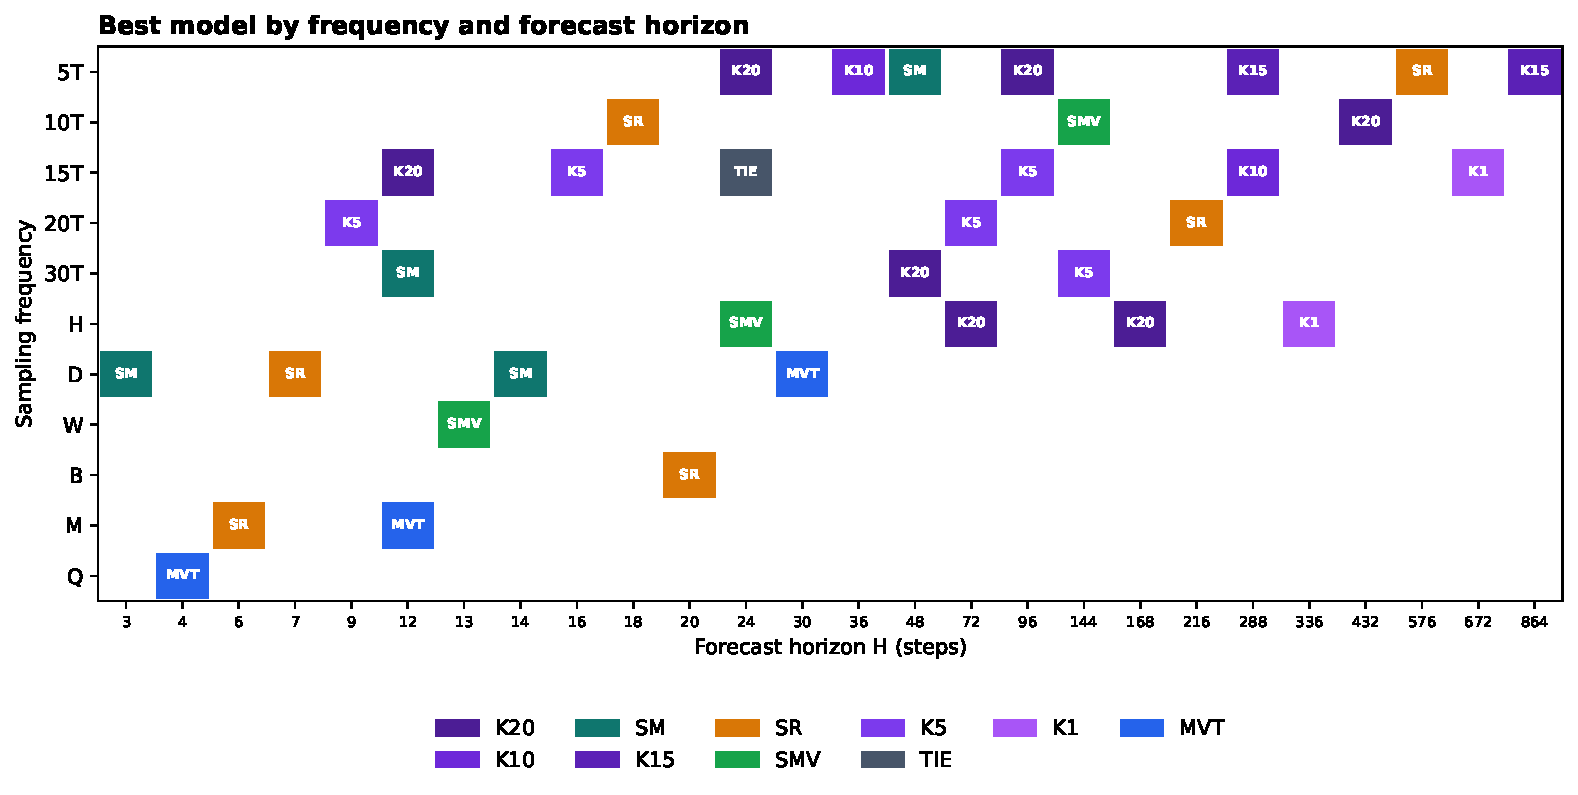
\includegraphics[width=\textwidth]{assets/best_model_heatmap.pdf}
\caption{Best completed pre-gate method at each sampling-frequency and
forecast-horizon cell, using the same tasks inside each cell. Codes: MVT native
multivariate; SM/SMV task/per-variate scope mix; SR scope ridge; K$x$ retrieval
mixture; TIE exact tie between univariate and scope selector. Sparse cells may
represent only one task.}
\end{figure}

\begin{figure}[p]
\centering
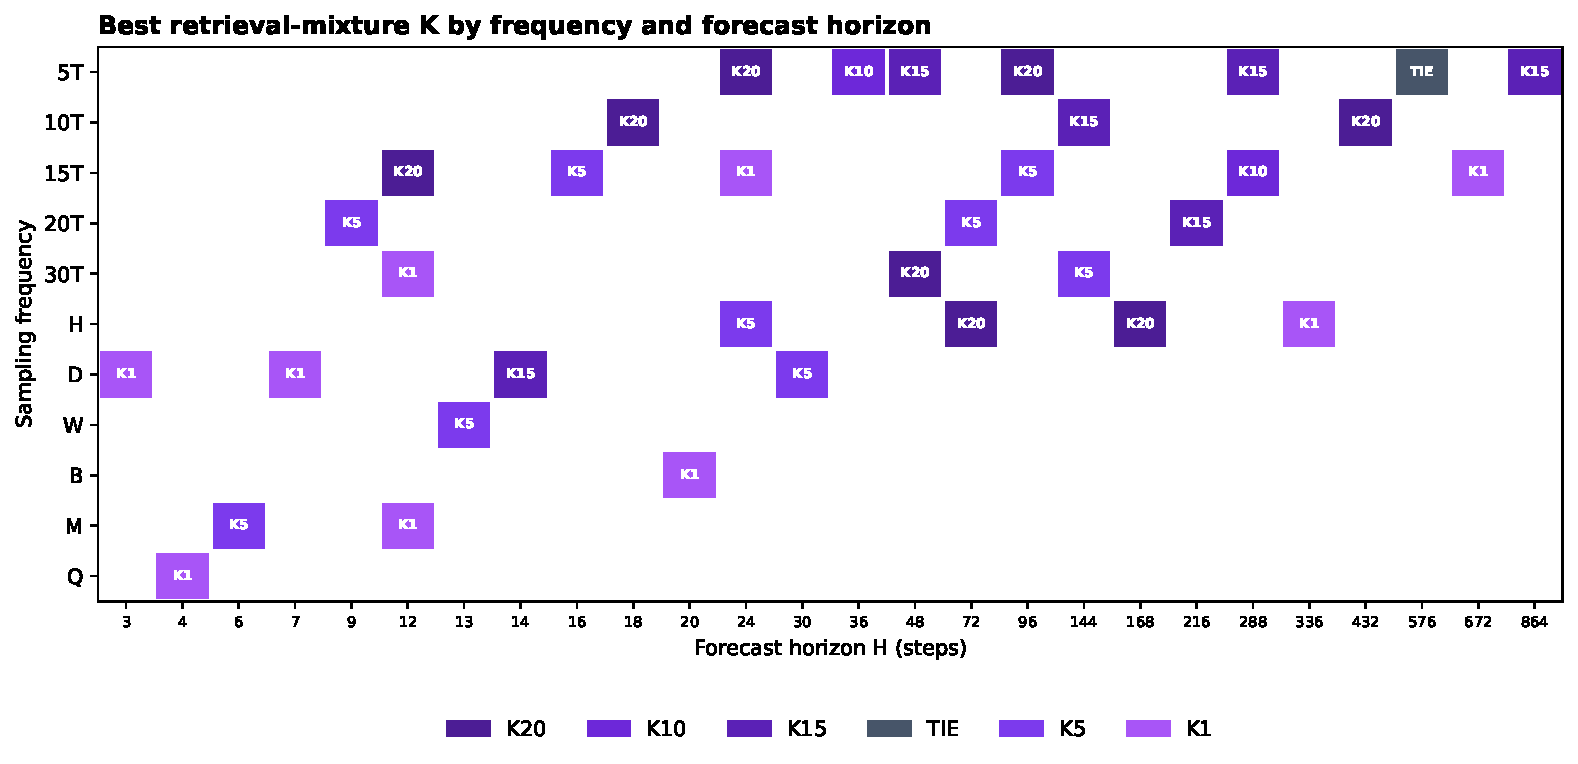
\includegraphics[width=\textwidth]{assets/best_k_heatmap.pdf}
\caption{Best $K$ when comparing only the five retrieval mixtures. Across 35
cells, $K=1$ and $K=5$ each win nine, $K=20$ wins eight, $K=15$ wins six,
$K=10$ wins two, and one cell ties. Aggregate $K=5$ is therefore a practical
default, not a universal optimum.}
\end{figure}

\section{Retrieval mixtures and fallback}

\begin{center}
\small
\begin{tabular}{rrrrrr}
\toprule
$K$ & Mean MASE & Improvement & Win/loss/tie & Same-series neighbors & Norm. calendar lag\\
\midrule
1 & 1.067750 & +0.138\% & 48/32/10 & 46.3\% & 0.450\\
5 & \textbf{1.065347} & \textbf{+0.363\%} & 51/29/10 & 43.9\% & 0.459\\
10 & 1.068043 & +0.111\% & 48/32/10 & 41.9\% & 0.469\\
15 & 1.068782 & +0.042\% & 50/30/10 & 40.3\% & 0.475\\
20 & 1.067474 & +0.164\% & 49/31/10 & 38.9\% & 0.479\\
\bottomrule
\end{tabular}
\end{center}

All five mixtures had a 4.612\% active retrieval fallback rate. For $K=5$,
the raw candidate lacked enough neighbors on 10,293 rows. Ten tasks already
had $p=0$ because they had no usable validation rows, so only 3,113 unavailable
test rows had a scientifically active nonzero retrieval weight and counted as
assembled-method fallback.

\begin{center}
\small
\begin{tabularx}{\textwidth}{@{}lllX@{}}
\toprule
Mixture state & Intended forecast & Unavailable alternative & Fallback count\\
\midrule
$p=0$ & $V$ & Alternative is unused & No: output was already exactly $V$\\
$p\ne0$ & $(1-p)V+pR$ & Emit $V$ & Yes: the intended mixture could not be formed\\
\bottomrule
\end{tabularx}
\end{center}

\section{Calibration distribution and new safeguards}

\begin{figure}[H]
\centering
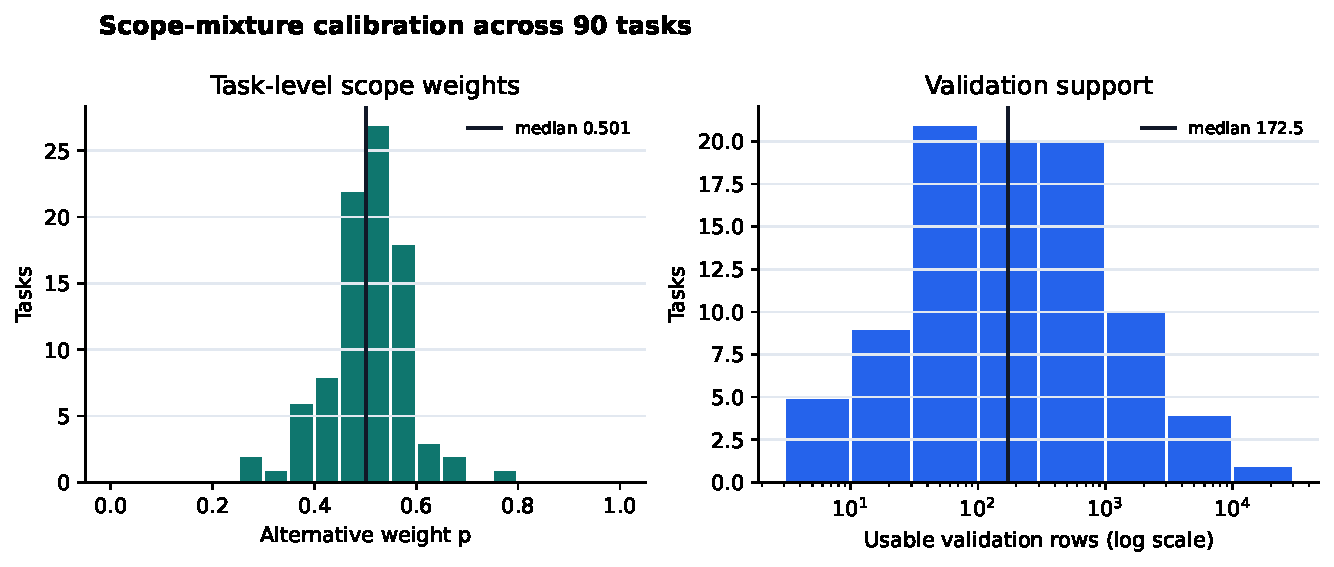
\includegraphics[width=.96\textwidth]{assets/scope_calibration.pdf}
\caption{Completed pre-gate task-scope calibration. The weight median is 0.501
(IQR 0.470--0.554; range 0.281--0.787). Usable validation rows have median
172.5 (IQR 41.25--519.75; range 4--14,868). The hard task selector separately
chose multivariate on 29 tasks and univariate on 61.}
\end{figure}

Beta smoothing alone assigns nonzero weight after zero observed wins. The new
gates make that prior contribution ineligible and also reject poorly supported
calibrations:

\begin{center}
\small
\begin{tabular}{rrrrl}
\toprule
Usable $n$ & Wins $w$ & Ungated Beta $p$ & Current $p$ & Reason\\
\midrule
1 & 0 & 33.33\% & 0 & $n<10$ and no wins\\
5 & 0 & 14.29\% & 0 & $n<10$ and no wins\\
10 & 0 & 8.33\% & 0 & $w/n\le10\%$\\
20 & 0 & 4.55\% & 0 & $w/n\le10\%$\\
50 & 0 & 1.92\% & 0 & $w/n\le10\%$\\
\bottomrule
\end{tabular}
\end{center}

The relative-support gate additionally requires $n/N_{\mathrm{test}}>10\%$.
At task level, the completed snapshot had no empirical win rate at or below
10\%; the support gate can still change low-$n$ tasks. At per-variate level,
240 of 3,882 completed selections had positive support but empirical win rate
at or below 10\%, so the new global gate is not result-neutral.

\section{Why the earlier convex and direct-horizon methods differ}

\begin{center}
\small
\begin{tabularx}{\textwidth}{@{}p{25mm}XX@{}}
\toprule
Property & Archived Adaptation convex fit & Selectime scope mix\\
\midrule
Forecast & $\lambda_0V+\sum_m\lambda_mZ_m$ & $(1-p)V+pM$\\
Parameters & $p+1$ simplex weights; eight for full $K=3$ & One scalar per task or item/variate\\
Fit target & Constrained least squares on pooled T1+T2 & Validation-window MSSE win frequency\\
Regularization & Simplex only; no ridge penalty & Beta smoothing plus current eligibility gates\\
Observed evidence & $-0.05\%$ to $+0.88\%$; below matched ridge & Pre-gate +0.932\% task and +1.013\% per-variate\\
Interpretation & More parameters may overfit, but candidates, splits, losses and datasets also differ & Simpler probability-like weight; not an MSSE-optimal coefficient\\
\bottomrule
\end{tabularx}
\end{center}

The older Selectime \texttt{top1\_horizon\_mix} was different again: it
blended $V$ directly with the rescaled observed continuation of the single
nearest neighbor and bypassed the backbone. One task produced a six-order-of-
magnitude failure; even after removing that task, the method did not beat
vanilla. The current $R_K$ instead results from in-model covariate conditioning
on $K$ retrieved examples before the outer mixture.

\section{Chronos-Bolt and timing boundary}

\begin{center}
\small
\begin{tabular}{lrrrr}
\toprule
Bolt method & Tasks & Mean MASE & Scaled MASE & Wins vs C2 univariate\\
\midrule
Vanilla univariate & 90 & 1.167905 & 0.776717 & 8/90\\
\bottomrule
\end{tabular}
\end{center}

Chronos-Bolt cannot produce $R_K$: its adapter rejects covariates and
multivariate histories. Treating neighbors as a batch would still forecast
them independently and would not condition the query on them. A post-hoc
neighbor-horizon mixture would be a new model-agnostic method, not the current
Selectime top-$K$ method.

The archived Adaptime timing path was designed to launch a fresh process for
each method and example, without cached predictions, representations or
neighbors. It was never run to a synchronized result. Current selected-method
latencies therefore remain undefined; recorded candidate query-loop times and
artifact-reuse overhead are not cold inference benchmarks.

\section{Rerun and future experiments}

\begin{center}
\small
\begin{tabularx}{\textwidth}{@{}p{36mm}p{39mm}X@{}}
\toprule
Rerun case & Estimated compute time & Evidence and boundary\\
\midrule
Chronos-2 gate-only refresh & 15--30 minutes, excluding queue & Reuse validation/test candidate forecasts; rerun calibration, assembly, evaluation and report. Previous calibration alone took about 90 seconds.\\
Cold Chronos-2 full workflow & 6--8 hours & The completed launch spent about 3 h 45 min in remaining validation prediction and was still in remaining test prediction more than 5 h 45 min after start.\\
Chronos-Bolt & No gate-driven rerun & It has no mixture calibration.\\
TS-ICL & Not yet estimable reliably & Depends on the terminal reusable candidate coverage of the current recovery.\\
\bottomrule
\end{tabularx}
\end{center}

Three follow-up studies are scientifically motivated but have not been run:

\begin{enumerate}
  \item \textbf{Gate refresh.} Regenerate the reduced Selectime comparison
  under the $n$, support-ratio and empirical-win gates before promoting any
  pre-gate number to the current result.
  \item \textbf{One-axis retrieval ablations on the best retrieval model.}
  Fix Chronos-2 \texttt{top\_k\_5\_mix}, then vary one TS-RAG-like choice at a
  time: all-series versus same-series scope, aligned versus unrestricted dates,
  instance-$L_2$ versus the alternative representation/distance, and
  query-scale rescaling versus its removal. This separates which retrieval
  choice matters while keeping $K=5$ fixed.
  \item \textbf{Test-fit oracles.} Fit the task/per-variate selector, mixture
  weight, and ridge coefficient directly on the test losses. These are not
  deployable forecasts: they intentionally leak test labels. Their value is an
  optimistic upper bound on the improvement available from perfect selection
  or calibration among the already computed candidates. Report both the oracle
  score and the gap from validation-fitted performance.
\end{enumerate}

\section{Limits}

The completed comparison uses one deterministic seed and provides no
across-run uncertainty or significance test. Frequency--horizon cells and
domains have unequal and sometimes very small task counts. The new gates are
implemented but unevaluated, so starred mixture values are not current gated
results. The proposed test-fit oracles would be diagnostic upper bounds only,
not honest model estimates. These limits preserve the descriptive value of the
completed snapshot while defining the exact rerun needed next.

\end{document}
